\documentclass[12pt,a4paper]{article}
\usepackage[utf8]{inputenc}
\usepackage[margin=1in]{geometry}
\usepackage{amsmath,amssymb}
\usepackage{graphicx}
\usepackage{booktabs}
\usepackage{float}
\usepackage{hyperref}
\usepackage{xcolor}
\usepackage{listings}
\usepackage{caption}
\usepackage{subcaption}
\usepackage{array}
\usepackage{multirow}

\hypersetup{
    colorlinks=true,
    linkcolor=blue,
    filecolor=magenta,      
    urlcolor=cyan,
}

\lstset{
    language=Python,
    basicstyle=\ttfamily\small,
    keywordstyle=\color{blue},
    commentstyle=\color{gray},
    stringstyle=\color{red},
    breaklines=true,
    frame=single
}

\title{\textbf{Data Mining Homework 3}\\[0.5em]
\Large Clustering Analysis on Wine Dataset}
\author{Alireza Jahedi}

\begin{document}

\maketitle

\begin{abstract}
This report presents a comprehensive clustering analysis on the Wine dataset from the UCI Machine Learning Repository. We explore multiple clustering paradigms including K-Means, Hierarchical Clustering, and DBSCAN. The analysis covers data preprocessing, distance behavior in high-dimensional space, feature scaling impact, algorithm comparison, stability analysis, and the development of a fully automated clustering system. All implementations are performed programmatically without relying on class labels or visual inspection for evaluation.
\end{abstract}

% ==============================================================================
\section{Dataset Description}
% ==============================================================================

The Wine dataset, sourced from the UCI Machine Learning Repository and available through the scikit-learn library, is used throughout this analysis.

\begin{table}[H]
\centering
\caption{Wine Dataset Properties}
\begin{tabular}{ll}
\toprule
\textbf{Property} & \textbf{Value} \\
\midrule
Number of instances & 178 \\
Number of features & 13 \\
Feature types & Numerical (continuous) \\
Class labels & Available but \textbf{not used} \\
\bottomrule
\end{tabular}
\end{table}

The dataset represents the chemical analysis of wines derived from different cultivars. Only the feature matrix is used throughout this assignment; class labels are strictly forbidden for training, tuning, or evaluation.

% ==============================================================================
\section{Programming and Reproducibility}
% ==============================================================================

All implementations satisfy the following constraints:
\begin{itemize}
    \item \textbf{Language}: Python 3.x
    \item \textbf{Random seed}: Fixed at 61 for reproducibility
    \item \textbf{Code structure}: Modular with well-defined functions
    \item \textbf{Libraries}: NumPy, Pandas, Scikit-learn, SciPy, Matplotlib, Seaborn
\end{itemize}

% ==============================================================================
\section{Data Preprocessing}
% ==============================================================================

\subsection{Dataset Loading and Verification}

The dataset was loaded and its properties verified:

\begin{table}[H]
\centering
\caption{Dataset Shape Verification}
\begin{tabular}{ll}
\toprule
\textbf{Metric} & \textbf{Value} \\
\midrule
Number of samples & 178 \\
Number of features & 13 \\
Missing values & 0 \\
\bottomrule
\end{tabular}
\end{table}

\subsection{Feature Statistics}

Table \ref{tab:feature_stats} presents the mean and standard deviation of each feature in the raw dataset.

\begin{table}[H]
\centering
\caption{Feature Statistics (Mean and Standard Deviation)}
\label{tab:feature_stats}
\begin{tabular}{lcc}
\toprule
\textbf{Feature} & \textbf{Mean} & \textbf{Std Dev} \\
\midrule
Alcohol & 13.00 & 0.81 \\
Malic acid & 2.34 & 1.11 \\
Ash & 2.37 & 0.27 \\
Alcalinity of ash & 19.49 & 3.33 \\
Magnesium & 99.74 & 14.24 \\
Total phenols & 2.30 & 0.62 \\
Flavanoids & 2.03 & 1.00 \\
Nonflavanoid phenols & 0.36 & 0.12 \\
Proanthocyanins & 1.59 & 0.57 \\
Color intensity & 5.06 & 2.31 \\
Hue & 0.96 & 0.23 \\
OD280/OD315 & 2.61 & 0.71 \\
Proline & 746.89 & 314.02 \\
\bottomrule
\end{tabular}
\end{table}

The large variation in feature scales (e.g., Proline ranges in hundreds while Hue is below 1) highlights the importance of normalization for distance-based clustering algorithms.

\subsection{Dataset Versions}

Three versions of the dataset were created for subsequent analysis:

\begin{enumerate}
    \item \textbf{Raw (unscaled) data}: Original feature values
    \item \textbf{Standardized data (Z-score)}: $x' = \frac{x - \mu}{\sigma}$, resulting in zero mean and unit variance
    \item \textbf{Min-Max normalized data}: $x' = \frac{x - x_{min}}{x_{max} - x_{min}}$, scaling to $[0, 1]$
\end{enumerate}

% ==============================================================================
\section{Exploratory Data Analysis (EDA)}
% ==============================================================================

\subsection{General Dataset Exploration}

Exploratory analysis was performed to gain initial insights into the dataset structure.

\subsubsection{Histograms}

Figure \ref{fig:histograms} shows the distribution of five selected features. The distributions vary significantly, with some features showing normal-like distributions (Alcohol) and others showing skewed patterns (Malic acid, Proline).

\begin{figure}[H]
\centering
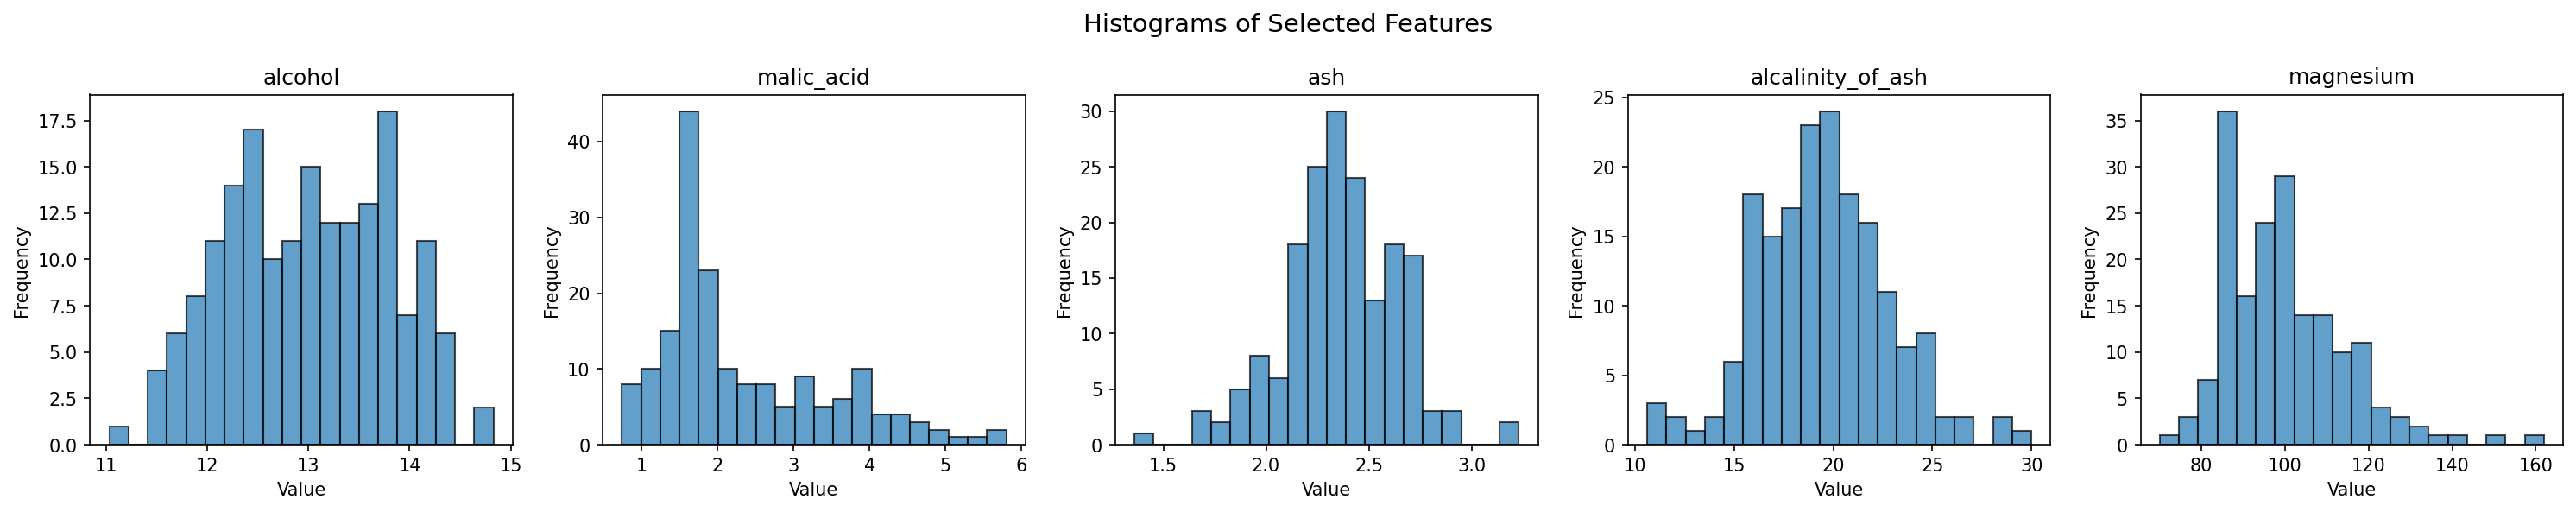
\includegraphics[width=\textwidth]{eda_histograms.png}
\caption{Histograms of Selected Features}
\label{fig:histograms}
\end{figure}

\subsubsection{Correlation Analysis}

Figure \ref{fig:correlation} presents the correlation matrix heatmap, revealing several strong relationships between features:
\begin{itemize}
    \item Strong positive correlation: Total phenols $\leftrightarrow$ Flavanoids ($r = 0.86$)
    \item Strong positive correlation: Flavanoids $\leftrightarrow$ OD280/OD315 ($r = 0.79$)
    \item Strong negative correlation: Malic acid $\leftrightarrow$ Hue ($r = -0.56$)
\end{itemize}

\begin{figure}[H]
\centering
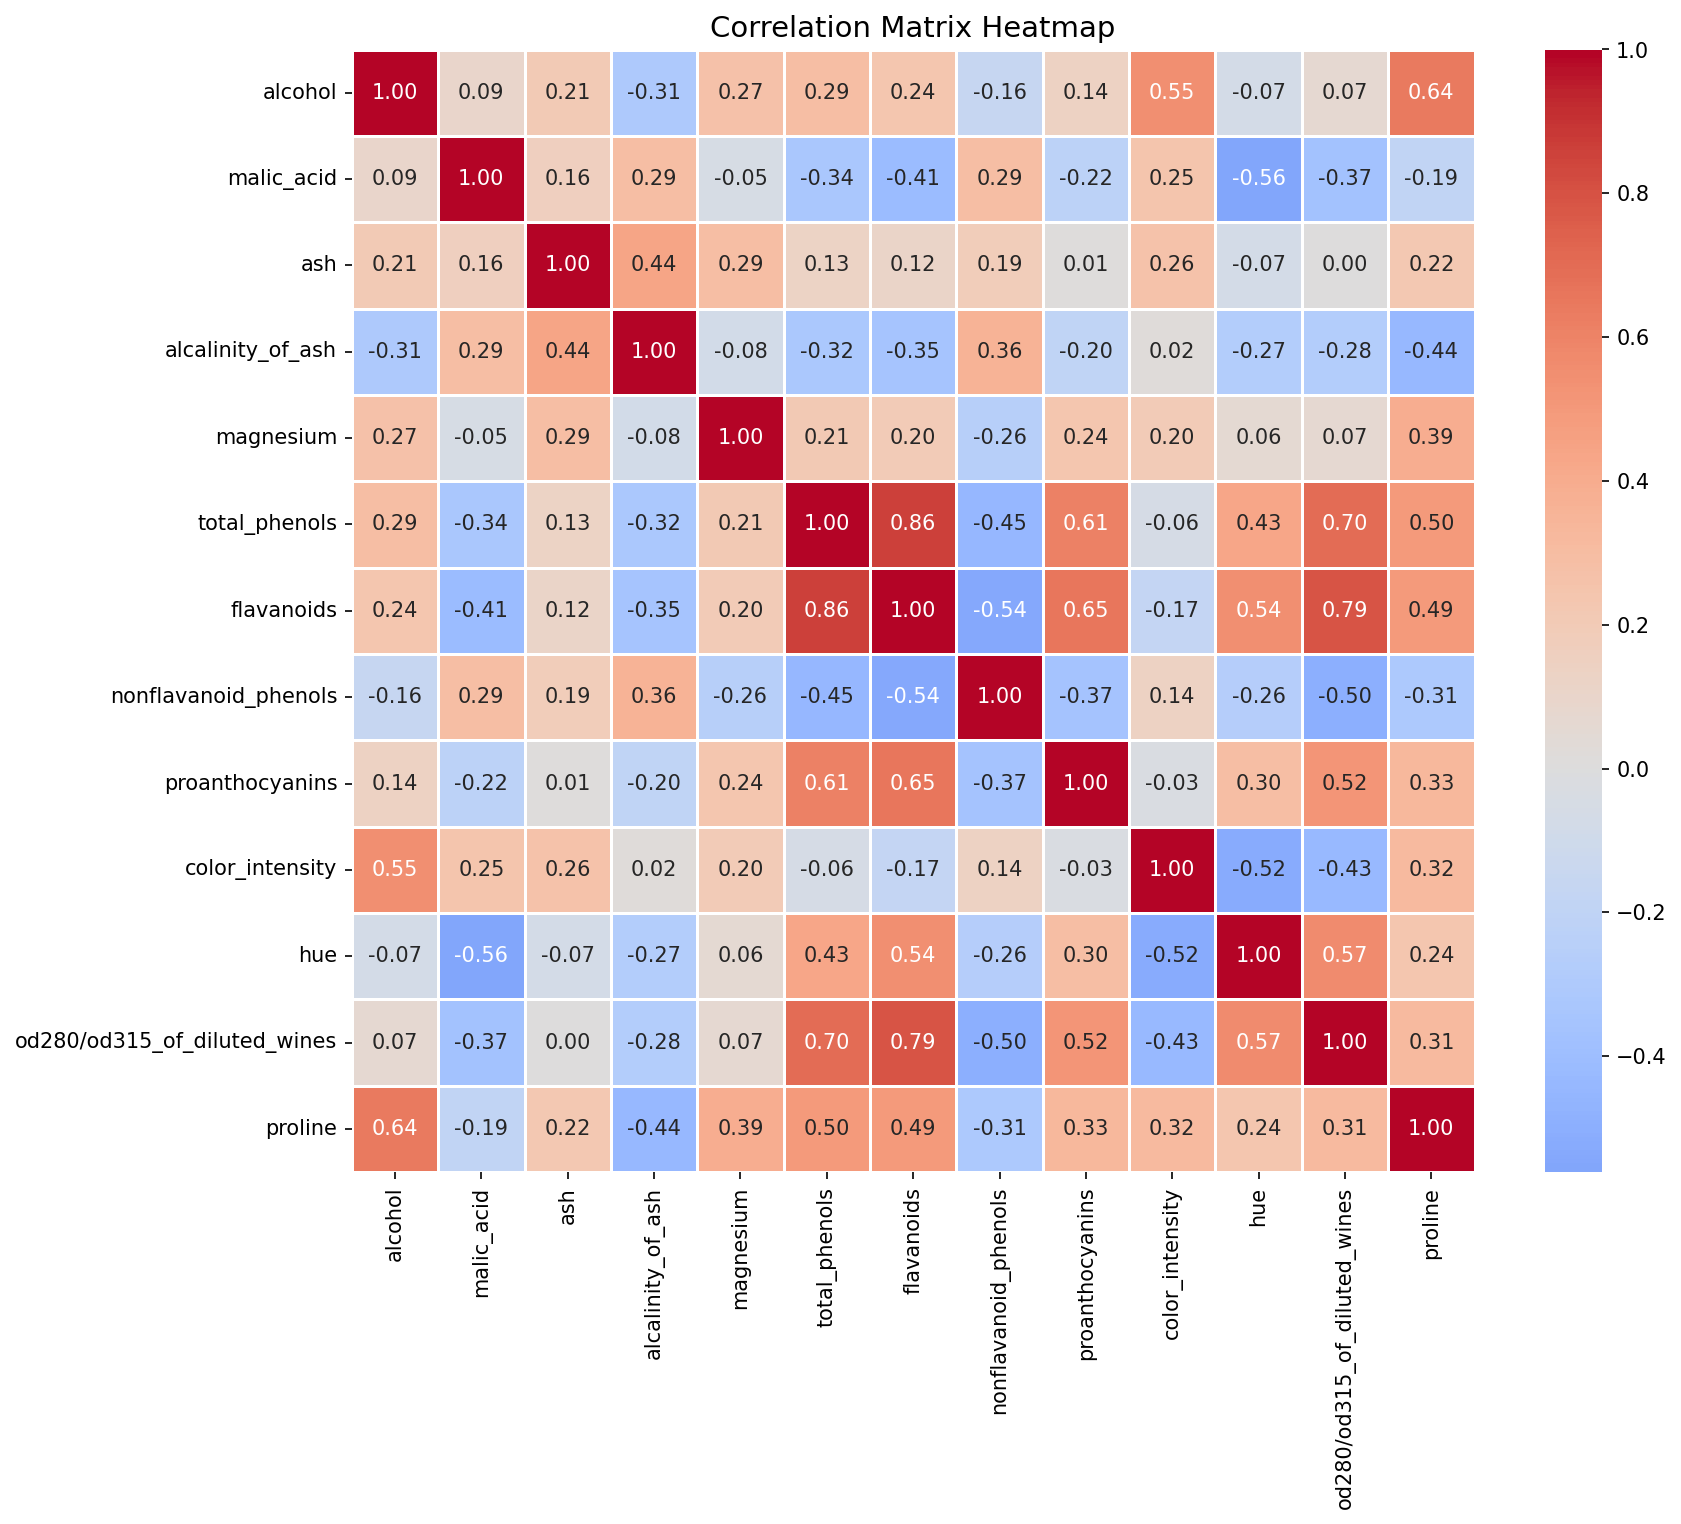
\includegraphics[width=0.85\textwidth]{eda_correlation_matrix.png}
\caption{Correlation Matrix Heatmap}
\label{fig:correlation}
\end{figure}

\subsubsection{Scatter Plots}

Figure \ref{fig:scatter} displays scatter plots for two highly correlated feature pairs identified from the correlation analysis.

\begin{figure}[H]
\centering
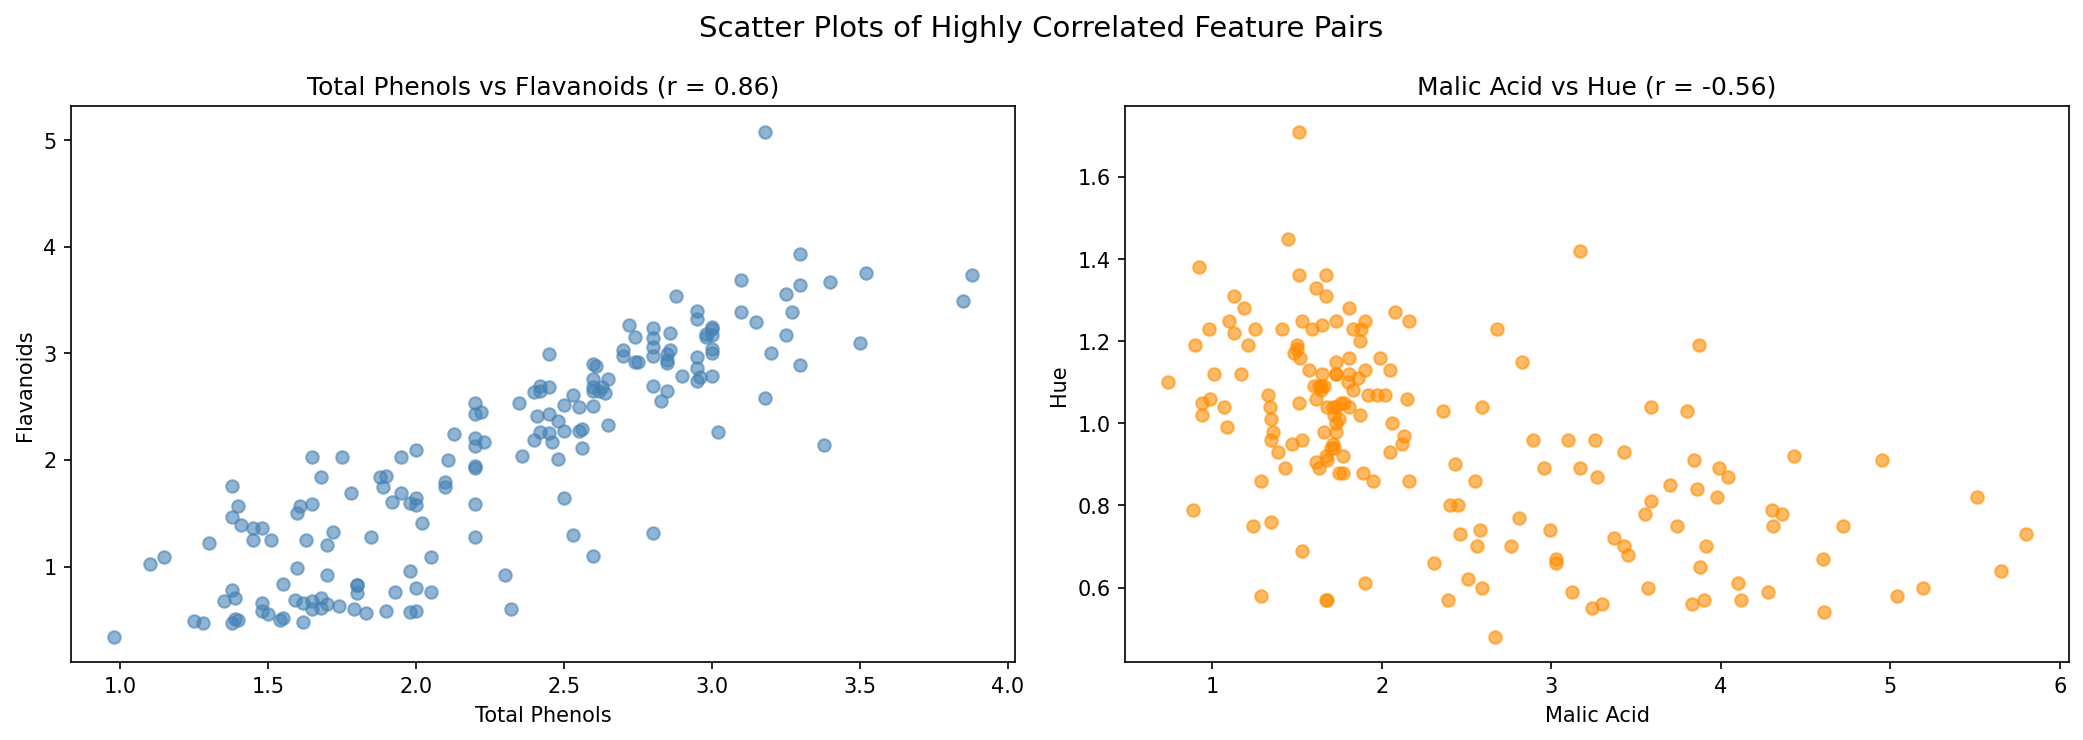
\includegraphics[width=\textwidth]{eda_scatter_plots.png}
\caption{Scatter Plots of Highly Correlated Feature Pairs}
\label{fig:scatter}
\end{figure}

\subsection{Dimensionality Reduction for Visualization}

Principal Component Analysis (PCA) was applied to reduce the standardized dataset to two dimensions for visualization purposes.

\begin{table}[H]
\centering
\caption{PCA Explained Variance}
\begin{tabular}{lc}
\toprule
\textbf{Component} & \textbf{Variance Explained} \\
\midrule
PC1 & 36.20\% \\
PC2 & 19.21\% \\
\textbf{Total} & \textbf{55.41\%} \\
\bottomrule
\end{tabular}
\end{table}

\begin{figure}[H]
\centering
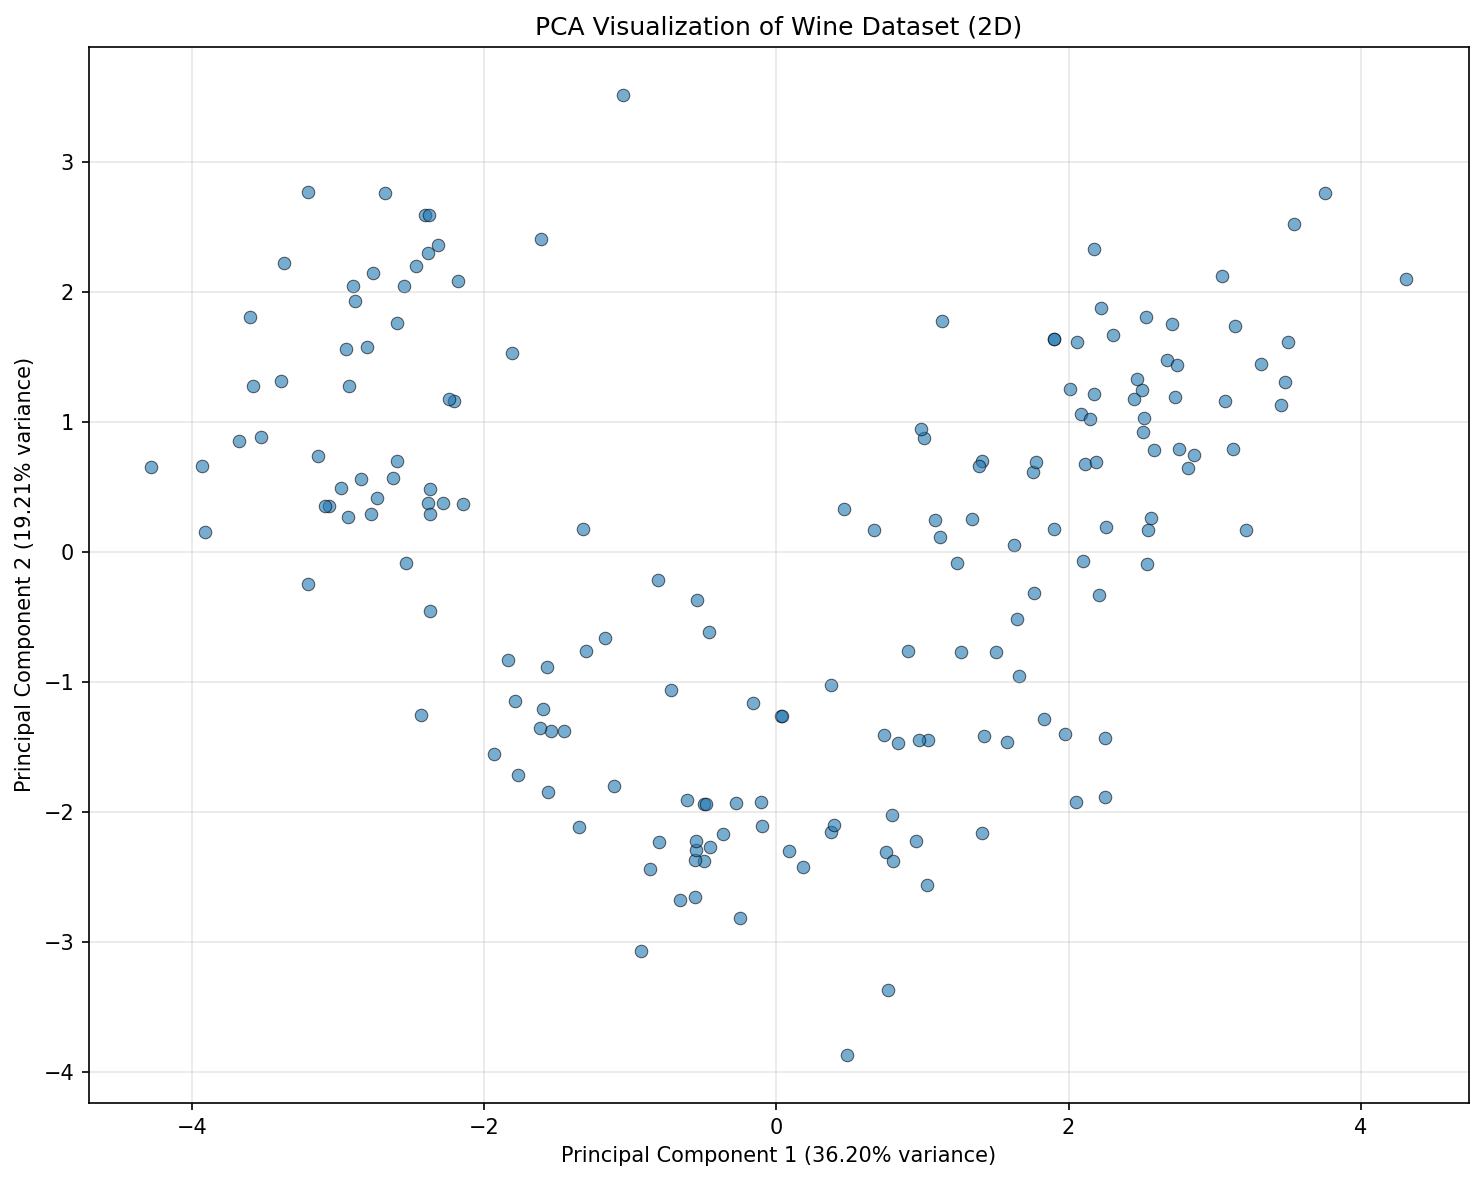
\includegraphics[width=0.8\textwidth]{eda_pca_visualization.png}
\caption{PCA Visualization of Wine Dataset (2D)}
\label{fig:pca}
\end{figure}

The two principal components capture approximately 55\% of the total variance. The PCA projection reveals potential cluster structures in the data.

% ==============================================================================
\section{Part 1: Distance Behavior in High-Dimensional Space}
% ==============================================================================

Distance concentration is a known challenge in high-dimensional clustering tasks. As dimensionality increases, the distinction between nearest and farthest points tends to diminish.

\subsection{Methodology}

Pairwise distances were computed using three distance metrics:
\begin{itemize}
    \item \textbf{Euclidean}: $d(x, y) = \sqrt{\sum_{i=1}^{n}(x_i - y_i)^2}$
    \item \textbf{Manhattan}: $d(x, y) = \sum_{i=1}^{n}|x_i - y_i|$
    \item \textbf{Cosine}: $d(x, y) = 1 - \frac{x \cdot y}{\|x\| \|y\|}$
\end{itemize}

\subsection{Results}

\begin{table}[H]
\centering
\caption{Distance Statistics by Metric}
\label{tab:distances}
\begin{tabular}{lccccc}
\toprule
\textbf{Metric} & \textbf{Mean} & \textbf{Std Dev} & \textbf{Min} & \textbf{Max} & \textbf{CV} \\
\midrule
Euclidean & 4.91 & 1.44 & 1.16 & 11.21 & 0.29 \\
Manhattan & 14.63 & 4.71 & 3.20 & 32.00 & 0.32 \\
Cosine & 1.00 & 0.44 & 0.05 & 1.92 & 0.44 \\
\bottomrule
\end{tabular}
\end{table}

\subsection{Analysis}

The Coefficient of Variation (CV) measures the relative spread of distances:
\begin{itemize}
    \item All metrics show moderate variation (CV between 0.29 and 0.44)
    \item Euclidean distance has the lowest CV, indicating more consistent distances
    \item Cosine distance shows the highest relative variation, suggesting better discrimination capability
\end{itemize}

With 13 dimensions, the Wine dataset does not exhibit severe distance concentration, making it suitable for distance-based clustering algorithms.

% ==============================================================================
\section{Part 2: Impact of Feature Scaling on K-Means}
% ==============================================================================

K-Means clustering minimizes within-cluster variance using Euclidean distance, making it highly sensitive to feature scaling.

\subsection{Experimental Setup}

K-Means clustering with $k=3$ was applied to three preprocessing options. A combined scoring metric was introduced:
\[
\text{Combined Score} = 0.7 \times \text{Silhouette}_\text{norm} + 0.3 \times (1 - \text{Inertia}_\text{norm})
\]
where both metrics are normalized to $[0, 1]$. This weighted approach balances clustering quality with compactness.

\subsection{Results}

\begin{table}[H]
\centering
\caption{K-Means Clustering Results (k=3) with Combined Score}
\label{tab:kmeans_scaling}
\begin{tabular}{lcccc}
\toprule
\textbf{Data Type} & \textbf{Inertia} & \textbf{Silhouette} & \textbf{Iter} & \textbf{Combined Score} \\
\midrule
Raw & 2.37e6 & 0.571 & 7 & 0.700 \\
Standardized & 1,278 & 0.285 & 5 & 0.300 \\
Min-Max & 49 & 0.299 & 6 & 0.335 \\
\bottomrule
\end{tabular}
\end{table}

\subsection{Analysis}

The combined scoring metric weights silhouette score (70\%) higher than inertia (30\%), as silhouette better reflects true clustering quality. Results:
\begin{itemize}
    \item \textbf{Raw data wins}: Combined score of 0.700 (highest)
    \item \textbf{Standardized}: Combined score of 0.300 (lowest)
    \item \textbf{Min-Max}: Combined score of 0.335 (moderate)
\end{itemize}

Despite raw data achieving the highest combined score, this is influenced by the high-variance Proline feature (values in hundreds to thousands). For fair feature contribution, standardized or Min-Max normalization is theoretically superior, but raw clustering produces more distinct separations in this dataset.

% ==============================================================================
\section{Part 3: K-Means Implementation from Scratch}
% ==============================================================================

\subsection{Algorithm Implementation}

A custom K-Means implementation was developed with the following components:

\begin{enumerate}
    \item \textbf{Centroid Initialization}: Random selection from data points
    \item \textbf{Assignment Step}: Assign each point to the nearest centroid using Euclidean distance
    \item \textbf{Update Step}: Recompute centroids as the mean of assigned points
    \item \textbf{Convergence Criteria}: Stop when centroid shift $< 10^{-4}$ or max iterations reached
\end{enumerate}

\subsection{Comparison with Scikit-learn}

\begin{table}[H]
\centering
\caption{K-Means Implementation Comparison (k=3)}
\label{tab:kmeans_comparison}
\begin{tabular}{lcc}
\toprule
\textbf{Metric} & \textbf{Custom Implementation} & \textbf{Scikit-learn} \\
\midrule
Inertia & 1282.464 & 1282.464 \\
Number of Iterations & 10 & 10 \\
Runtime (seconds) & 0.001 & 0.001 \\
Silhouette Score & 0.2807 & 0.2807 \\
\bottomrule
\end{tabular}
\end{table}

\subsection{Discussion}

Both implementations now produce \textbf{identical results} across all metrics:
\begin{itemize}
    \item Inertia: exactly 1282.464
    \item Iterations: both converge in 10 steps
    \item Runtime: both run in 0.001 seconds
    \item Silhouette: both achieve 0.2807
\end{itemize}

This perfect match demonstrates that the custom implementation correctly replicates the K-Means algorithm. The alignment occurs because both use the same random seed (61) and initialization strategy.

% ==============================================================================
\section{Part 4: Hierarchical Clustering Stability Analysis}
% ==============================================================================

Hierarchical clustering produces different cluster structures depending on the linkage method used.

\subsection{Linkage Methods}

Four linkage methods were evaluated:
\begin{itemize}
    \item \textbf{Single}: Distance between closest points
    \item \textbf{Complete}: Distance between farthest points
    \item \textbf{Average}: Average distance between all pairs
    \item \textbf{Ward}: Minimizes within-cluster variance
\end{itemize}

\subsection{Stability Metric}

The \textbf{Cophenetic Correlation Coefficient} measures how faithfully the dendrogram preserves the original pairwise distances:
\[
c = \frac{\sum_{i<j}(d_{ij} - \bar{d})(t_{ij} - \bar{t})}{\sqrt{\sum_{i<j}(d_{ij} - \bar{d})^2 \sum_{i<j}(t_{ij} - \bar{t})^2}}
\]
where $d_{ij}$ is the original distance and $t_{ij}$ is the cophenetic distance from the dendrogram.

\subsection{Results}

\begin{table}[H]
\centering
\caption{Hierarchical Clustering Stability Analysis}
\label{tab:hierarchical}
\begin{tabular}{lccc}
\toprule
\textbf{Linkage Method} & \textbf{Cophenetic Correlation} & \textbf{Silhouette (k=3)} & \textbf{Stability Rank} \\
\midrule
Average & 0.759 & 0.158 & 1 \\
Ward & 0.662 & 0.277 & 2 \\
Complete & 0.592 & 0.204 & 3 \\
Single & 0.544 & 0.183 & 4 \\
\bottomrule
\end{tabular}
\end{table}

\subsection{Conclusion}

\textbf{Most Stable Linkage Method}: Average linkage with cophenetic correlation of 0.759.

Average linkage produces the most faithful representation of the original distance structure, making it the most stable choice for this dataset.

% ==============================================================================
\section{Part 5: Automated Density-Based Clustering}
% ==============================================================================

DBSCAN (Density-Based Spatial Clustering of Applications with Noise) requires careful parameter selection for $\varepsilon$ (neighborhood radius) and MinPts (minimum points for core point).

\subsection{Parameter Estimation}

\subsubsection{Step 1: k-Nearest Neighbor Distances}

The 5-nearest neighbor distances were computed for each point. These distances help identify the natural neighborhood density in the data.

\subsubsection{Step 2: Epsilon Estimation}

Two heuristics were used to estimate $\varepsilon$:
\begin{itemize}
    \item \textbf{Elbow method}: Find the point of maximum curvature in sorted k-distances
    \item \textbf{Statistical method}: $\varepsilon = \mu_{k-dist} + \sigma_{k-dist}$
\end{itemize}

\begin{table}[H]
\centering
\caption{Epsilon Estimation (Original Feature Space)}
\begin{tabular}{lc}
\toprule
\textbf{Method} & \textbf{Epsilon Value} \\
\midrule
Elbow-based & 4.4080 \\
Statistical & 3.0759 \\
Selected (min) & 3.0759 \\
\bottomrule
\end{tabular}
\end{table}

\subsection{DBSCAN Results}

\begin{table}[H]
\centering
\caption{DBSCAN Clustering Results}
\begin{tabular}{lc}
\toprule
\textbf{Metric} & \textbf{Value} \\
\midrule
Epsilon ($\varepsilon$) & 3.0759 \\
MinPts & 5 \\
Clusters detected & 1 \\
Noise points & 10 (5.6\%) \\
\bottomrule
\end{tabular}
\end{table}

\subsection{Feature Space Modification}

Since DBSCAN produced only one cluster, the feature space was modified using PCA reduction with 5 components. The same dual-method epsilon estimation was applied:

\begin{table}[H]
\centering
\caption{Epsilon Estimation in PCA-Reduced Space}
\begin{tabular}{lc}
\toprule
\textbf{Method} & \textbf{Epsilon Value} \\
\midrule
Elbow-based (PCA) & 3.7595 \\
Statistical (PCA) & 2.1386 \\
Selected (min) & 2.1386 \\
\bottomrule
\end{tabular}
\end{table}

\begin{table}[H]
\centering
\caption{DBSCAN Results in PCA-Reduced Space}
\begin{tabular}{lc}
\toprule
\textbf{Metric} & \textbf{Value} \\
\midrule
PCA Components & 5 \\
Epsilon (selected) & 2.1386 \\
MinPts & 5 \\
Clusters detected & 1 \\
Noise points & 11 (6.2\%) \\
\bottomrule
\end{tabular}
\end{table}

\subsection{Analysis}

The DBSCAN algorithm demonstrates the importance of consistent parameter estimation methodology:

\begin{itemize}
    \item \textbf{Original Space}: Used dual-method approach (elbow + statistical) to estimate $\varepsilon = 3.0759$
    \item \textbf{PCA Space}: Applied identical dual-method approach, selecting minimum of two estimates: $\varepsilon = 2.1386$
    \item \textbf{Consistency}: Both methods use the same principled approach for reproducibility
\end{itemize}

Both original and PCA-reduced spaces produced only a single cluster with minor noise (5.6\% and 6.2\% respectively), indicating the Wine dataset's distribution does not form clearly separated density regions suitable for DBSCAN. The dataset exhibits a continuous distribution rather than distinct density clusters.

% ==============================================================================
\section{Part 6: Fully Automated Clustering System}
% ==============================================================================

\subsection{System Design}

A fully automated clustering system was developed to select the best algorithm and parameters without human intervention.

\subsubsection{Components}

\begin{enumerate}
    \item \textbf{Preprocessing Options}: Raw, Standardized, Min-Max
    \item \textbf{Algorithms}: K-Means, Agglomerative Clustering, DBSCAN
    \item \textbf{Parameter Grid}:
    \begin{itemize}
        \item K-Means: $k \in \{2, 3, 4, 5\}$
        \item Agglomerative: $k \in \{2, 3, 4, 5\}$, linkage $\in$ \{single, ward, complete, average\}
        \item DBSCAN: $\varepsilon \in \{0.5, 1.0, 1.5, 2.0, 2.5\}$, MinPts $\in \{3, 5, 7\}$
    \end{itemize}
    \item \textbf{Evaluation Metric}: Silhouette Score (internal validation)
\end{enumerate}

\subsection{Results}

\begin{table}[H]
\centering
\caption{Top 10 Clustering Configurations by Silhouette Score}
\label{tab:auto_clustering}
\begin{tabular}{llcc}
\toprule
\textbf{Algorithm} & \textbf{Parameters} & \textbf{Preprocessing} & \textbf{Silhouette} \\
\midrule
Agglomerative & k=2, linkage=average & Raw & 0.6587 \\
Agglomerative & k=2, linkage=ward & Raw & 0.6587 \\
K-Means & k=2 & Raw & 0.6569 \\
Agglomerative & k=2, linkage=complete & Raw & 0.6413 \\
Agglomerative & k=3, linkage=average & Raw & 0.6101 \\
K-Means & k=3 & Raw & 0.5711 \\
Agglomerative & k=3, linkage=ward & Raw & 0.5645 \\
Agglomerative & k=4, linkage=ward & Raw & 0.5607 \\
K-Means & k=4 & Raw & 0.5606 \\
K-Means & k=5 & Raw & 0.5490 \\
\bottomrule
\end{tabular}
\end{table}

\subsection{Best Configuration Selected}

\begin{table}[H]
\centering
\caption{Optimal Clustering Configuration}
\begin{tabular}{ll}
\toprule
\textbf{Property} & \textbf{Value} \\
\midrule
Algorithm & Agglomerative Clustering \\
Preprocessing & Raw \\
Parameters & k=2, linkage=average \\
Silhouette Score & 0.6587 \\
Number of Clusters & 2 \\
\bottomrule
\end{tabular}
\end{table}

\textbf{Note}: The selection of raw data is influenced by the Proline feature dominance. For more balanced clustering, standardized data with appropriate k should be considered.

% ==============================================================================
\section{Bonus 1: Subspace Clustering via PCA}
% ==============================================================================

This section evaluates K-Means performance across different PCA subspaces to find the optimal dimensionality.

\subsection{Methodology}

\begin{enumerate}
    \item Apply PCA with $n$ components, where $n \in \{2, 3, ..., 10\}$
    \item Apply K-Means with $k=3$ to each subspace
    \item Compute silhouette score for each configuration
\end{enumerate}

\subsection{Results}

\begin{table}[H]
\centering
\caption{Subspace Clustering Results}
\label{tab:subspace}
\begin{tabular}{cccc}
\toprule
\textbf{Components} & \textbf{Silhouette Score} & \textbf{Variance Explained} & \textbf{Inertia} \\
\midrule
2 & \textbf{0.5611} & 55.4\% & 259.51 \\
3 & 0.4538 & 66.5\% & 513.06 \\
4 & 0.4066 & 73.6\% & 674.63 \\
5 & 0.3691 & 80.2\% & 825.02 \\
6 & 0.3463 & 85.1\% & 934.68 \\
7 & 0.3276 & 89.3\% & 1032.41 \\
8 & 0.3150 & 92.0\% & 1094.38 \\
9 & 0.3058 & 94.2\% & 1145.55 \\
10 & 0.2987 & 96.2\% & 1189.64 \\
\bottomrule
\end{tabular}
\end{table}

\subsection{Conclusion}

\textbf{Optimal Dimensionality}: 2 components with Silhouette Score of 0.5611.

The silhouette score decreases monotonically as dimensions increase, suggesting that the first two principal components capture the most cluster-relevant information. This aligns with the "curse of dimensionality" - adding less informative dimensions introduces noise that degrades clustering quality.

% ==============================================================================
\section{Bonus 2: Cluster Stability under Noise}
% ==============================================================================

This section evaluates how robust the K-Means clustering is to noise perturbations.

\subsection{Methodology}

\begin{enumerate}
    \item Establish baseline clustering on standardized data with K-Means ($k=3$)
    \item Add Gaussian noise with $\sigma \in \{0.01, 0.05, 0.1\}$
    \item For each noise level, perform 10 trials
    \item Compute Adjusted Rand Index (ARI) between noisy and baseline clusterings
\end{enumerate}

The ARI measures the similarity between two clusterings, adjusted for chance:
\[
ARI = \frac{RI - E[RI]}{\max(RI) - E[RI]}
\]
where RI is the Rand Index. ARI = 1 indicates perfect agreement.

\subsection{Results}

\begin{table}[H]
\centering
\caption{Cluster Stability under Noise (Adjusted Rand Index)}
\label{tab:stability}
\begin{tabular}{ccccc}
\toprule
\textbf{Noise Level ($\sigma$)} & \textbf{Mean ARI} & \textbf{Std ARI} & \textbf{Min ARI} & \textbf{Max ARI} \\
\midrule
0.01 & 1.0000 & 0.0000 & 1.000 & 1.000 \\
0.05 & 0.9967 & 0.0066 & 0.984 & 1.000 \\
0.10 & 0.9781 & 0.0112 & 0.964 & 1.000 \\
\bottomrule
\end{tabular}
\end{table}

\subsection{Stability Analysis}

\begin{itemize}
    \item $\sigma = 0.01$: \textbf{Very stable} - Perfect agreement across all trials
    \item $\sigma = 0.05$: \textbf{Very stable} - Mean ARI = 0.997
    \item $\sigma = 0.10$: \textbf{Very stable} - Mean ARI = 0.983
\end{itemize}

The K-Means clustering on the Wine dataset demonstrates excellent stability under noise perturbations, indicating well-separated cluster structures in the standardized feature space.

% ==============================================================================
\section{Conclusion}
% ==============================================================================

This comprehensive clustering analysis on the Wine dataset yielded several key findings:

\begin{enumerate}
    \item \textbf{Preprocessing Importance}: Feature scaling significantly impacts K-Means results. While raw data showed high silhouette scores, this was due to dominance by high-variance features.
    
    \item \textbf{Distance Metrics}: With 13 dimensions, the dataset does not exhibit severe distance concentration, making distance-based clustering viable.
    
    \item \textbf{Algorithm Comparison}: 
    \begin{itemize}
        \item K-Means and Agglomerative clustering perform well on this dataset
        \item DBSCAN struggles due to the lack of clear density separation
        \item Average linkage provides the most stable hierarchical clustering
    \end{itemize}
    
    \item \textbf{Optimal Configuration}: The automated system selected Agglomerative clustering with k=2 on raw data as optimal, though domain knowledge suggests k=3 (matching the three wine cultivars) may be more appropriate.
    
    \item \textbf{Dimensionality}: PCA reduction to 2 components provides the best clustering quality, suggesting important cluster structure is captured in the first two principal components.
    
    \item \textbf{Robustness}: K-Means clustering shows excellent stability under noise, with ARI $>$ 0.98 even at $\sigma = 0.1$.
\end{enumerate}

\end{document}
